% sections/03-main.tex --- Виклад основного матеріалу.
% Covers PARCS-Agent architecture, MCP tool surface, layer execution model,
% and the Monte Carlo VaR case study.

\citsection{Main material and results}

\medskip\noindent\textbf{PARCS-Agent architecture}\par\nopagebreak
PARCS-Agent comprises three cooperating components: an MCP server, the existing PARCS Host and Daemon services, and a thin runtime contract shared between them. The MCP server is implemented as an ASP.NET Core service (\texttt{Parcs.Agent.Mcp}) deployed alongside the PARCS Host within the same Kubernetes namespace. It encapsulates five collaborating internal services: a \texttt{RoslynCompilerService}, which compiles agent-supplied source against the agent runtime contract; a \texttt{SessionManager}, which maintains compiled sessions and their layer history; a \texttt{ClusterInfoService}, which queries the Kubernetes API for current capacity; a \texttt{ParcsApiClient}, which submits jobs to the PARCS Host through its existing REST surface; and an \texttt{AgentRunnerModuleRegistrar} hosted service that registers the agent-runner module at start-up.

The agent does not communicate with the PARCS Host directly. All interaction proceeds through the MCP server, which simultaneously functions as a translation layer between MCP and PARCS job semantics and as a state owner for compiled sessions, layer outputs, and the dataset cache.

\begin{center}
\IfFileExists{figures/fig1-architecture.png}{%
    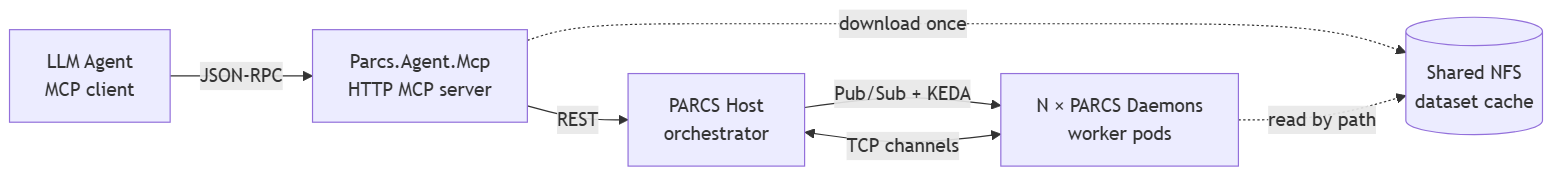
\includegraphics[width=0.85\linewidth]{figures/fig1-architecture}%
}{%
    \fbox{\parbox[c][6em][c]{0.85\linewidth}{\centering\footnotesize\itshape
        [Fig.~1 placeholder --- render \texttt{figures/fig1-architecture.mmd}
        to PNG/PDF and place at \texttt{figures/fig1-architecture.png}]}}%
}
\end{center}
\citfigcaption{1}{%
    \foreignlanguage{ukrainian}{Виконавчий потік PARCS-Agent: агент взаємодіє з MCP-сервером у Kubernetes, який компілює подану логіку, диспетчеризує її через PARCS Host і повертає результати.}%
}{%
    PARCS-Agent execution flow: the agent communicates with a Kubernetes-resident MCP server, which compiles agent-supplied code, dispatches it through the PARCS Host, and propagates results back. KEDA scales daemon pods on demand; bulk inputs traverse a shared NFS volume rather than the protocol.%
}

The architecture has two characteristic properties worth highlighting. First, all parallelism is encapsulated below the MCP boundary, so that the agent only observes synchronous tool invocations. Second, bulk input data does not transit the protocol: the MCP server retrieves a referenced URL once into a shared volume and provides each worker with an identical on-disk path, eliminating per-worker file replication that would otherwise occur.

\medskip\noindent\textbf{The MCP tool surface}\par\nopagebreak
The MCP server exposes four tools, summarised in Table~1. The tool definitions correspond directly to the production source \texttt{ParcsAgentTools.cs} in~\cite{bohusevych2026parcs}.

\cittabcaption{1}{%
    \foreignlanguage{ukrainian}{Інструменти MCP-сервера PARCS-Agent.}%
}{%
    PARCS-Agent MCP tool surface.%
}
\begin{center}
\small
\begin{tabularx}{\dimexpr\linewidth-1cm\relax}{|>{\raggedright\arraybackslash}p{2.6cm}|>{\raggedright\arraybackslash}X|>{\raggedright\arraybackslash}X|>{\raggedright\arraybackslash}X|}
\hline
\textbf{Tool} & \textbf{Purpose} & \textbf{Key inputs} & \textbf{Returns} \\
\hline
\texttt{get\_cluster\_info} & Capability discovery & --- & \texttt{\{workerNodeCount, maxParallelism, daemonCpuRequestMillicores\}} \\
\hline
\texttt{create\_session} & Compile and register an \texttt{IAgentComputation} class & \texttt{sourceCode} (C\#) & \texttt{\{sessionId\}} or \texttt{\{error\}} with diagnostics \\
\hline
\texttt{run\_layer} & Execute a layer in parallel; block until completion & \texttt{sessionId, parallelism, previousLayerId?, customData?, parameters?, datasetUrl?} & \texttt{\{layerId, status, totalElapsedSeconds, successCount, failureCount, result\}} \\
\hline
\texttt{list\_sessions} & Enumerate active sessions & --- & \texttt{[\{sessionId, createdAt, \dots\}]} \\
\hline
\end{tabularx}
\end{center}

The surface is deliberately minimal. There is no fire-and-forget execution variant of \texttt{run\_layer}, no explicit polling endpoint, and no client-side reduction primitive; each such addition would introduce concepts to the agent's prompt without enlarging the class of computations the agent is able to express. Three properties of the design merit explicit discussion.

\textit{Verbose tool descriptions as prompt content.}\quad Each tool's \texttt{[Description]} attribute provides explicit parameter bounds, example values, and the expected response contract. This design responds to the finding~\cite{luo2025mcpsmelly} that the majority of public MCP tools insufficiently document their parameters. The descriptions are concise enough to fit within typical LLM context windows, yet detailed enough to reduce the incidence of malformed agent calls.

\textit{Reference-based result passing.}\quad The \texttt{run\_layer} tool returns a \texttt{layerId}; subsequent layers reference prior outputs through \texttt{previousLayerId} rather than re-transmitting the full result payload. The MCP server retrieves the stored result internally and exposes it to each worker through \texttt{input.PreviousLayerResultJson}. Hence, potentially large JSON payloads are not sent through the LLM context twice --- once on the way out and once on the way back in. The response payload, in turn, returns \texttt{result} as a structured nested object rather than an escaped JSON string, eliminating Unicode-escaped quotes from string-in-string payloads and further reducing token consumption.

\textit{Failure semantics that preserve session state.}\quad A compilation error is reported as \texttt{\{error\}} from \texttt{create\_session} without affecting earlier sessions. A worker exception during \texttt{run\_layer} is reported with \texttt{status: "Failed"} and accompanying diagnostic detail, including a hint when the failure mode is recognisable (e.g. out-of-memory). The session itself remains usable; recovery proceeds by submitting corrected source through \texttt{create\_session} and resuming with the last successful \texttt{layerId} passed as \texttt{previousLayerId}. No prior work is lost. This semantics accommodates the observation that LLMs occasionally produce correct code only on a second attempt, in which case a less forgiving protocol would force redundant re-execution of already-completed work.

\medskip\noindent\textbf{The layer execution model}\par\nopagebreak
A computation is decomposed into a sequence of \emph{layers}. Each layer comprises a parallel fan-out across $N$ workers, a barrier, and a single aggregated JSON value that constitutes the input to the subsequent layer. This fan-out~/~barrier construct is the only execution primitive exposed to the agent; the protocol provides no direct support for point-to-point communication, scatter--gather, or shared memory.

The agent-side contract is the single-method interface \texttt{IAgentComputation} from \texttt{Parcs.Agent.Runtime}:

\begin{lstlisting}
public interface IAgentComputation
{
    Task<AgentLayerResult> ExecuteAsync(
        AgentLayerInput input, CancellationToken ct = default);
}
\end{lstlisting}

The \texttt{AgentLayerInput} type exposes the fields \texttt{WorkerIndex}, \texttt{TotalWorkers}, \texttt{PreviousLayerResultJson}, \texttt{CustomData}, \texttt{Parameters}, and \texttt{DatasetPath}; the worker returns either \texttt{AgentLayerResult.Ok(outputJson)} or \texttt{AgentLayerResult.Error(message)}. The body of \texttt{ExecuteAsync} is written by the agent as straight-line C\#, in the same paradigm as within a single-threaded sandbox. Fan-out, fan-in, JSON marshalling, and inter-worker isolation are the responsibility of the platform.

\begin{center}
\IfFileExists{figures/fig2-sequence.png}{%
    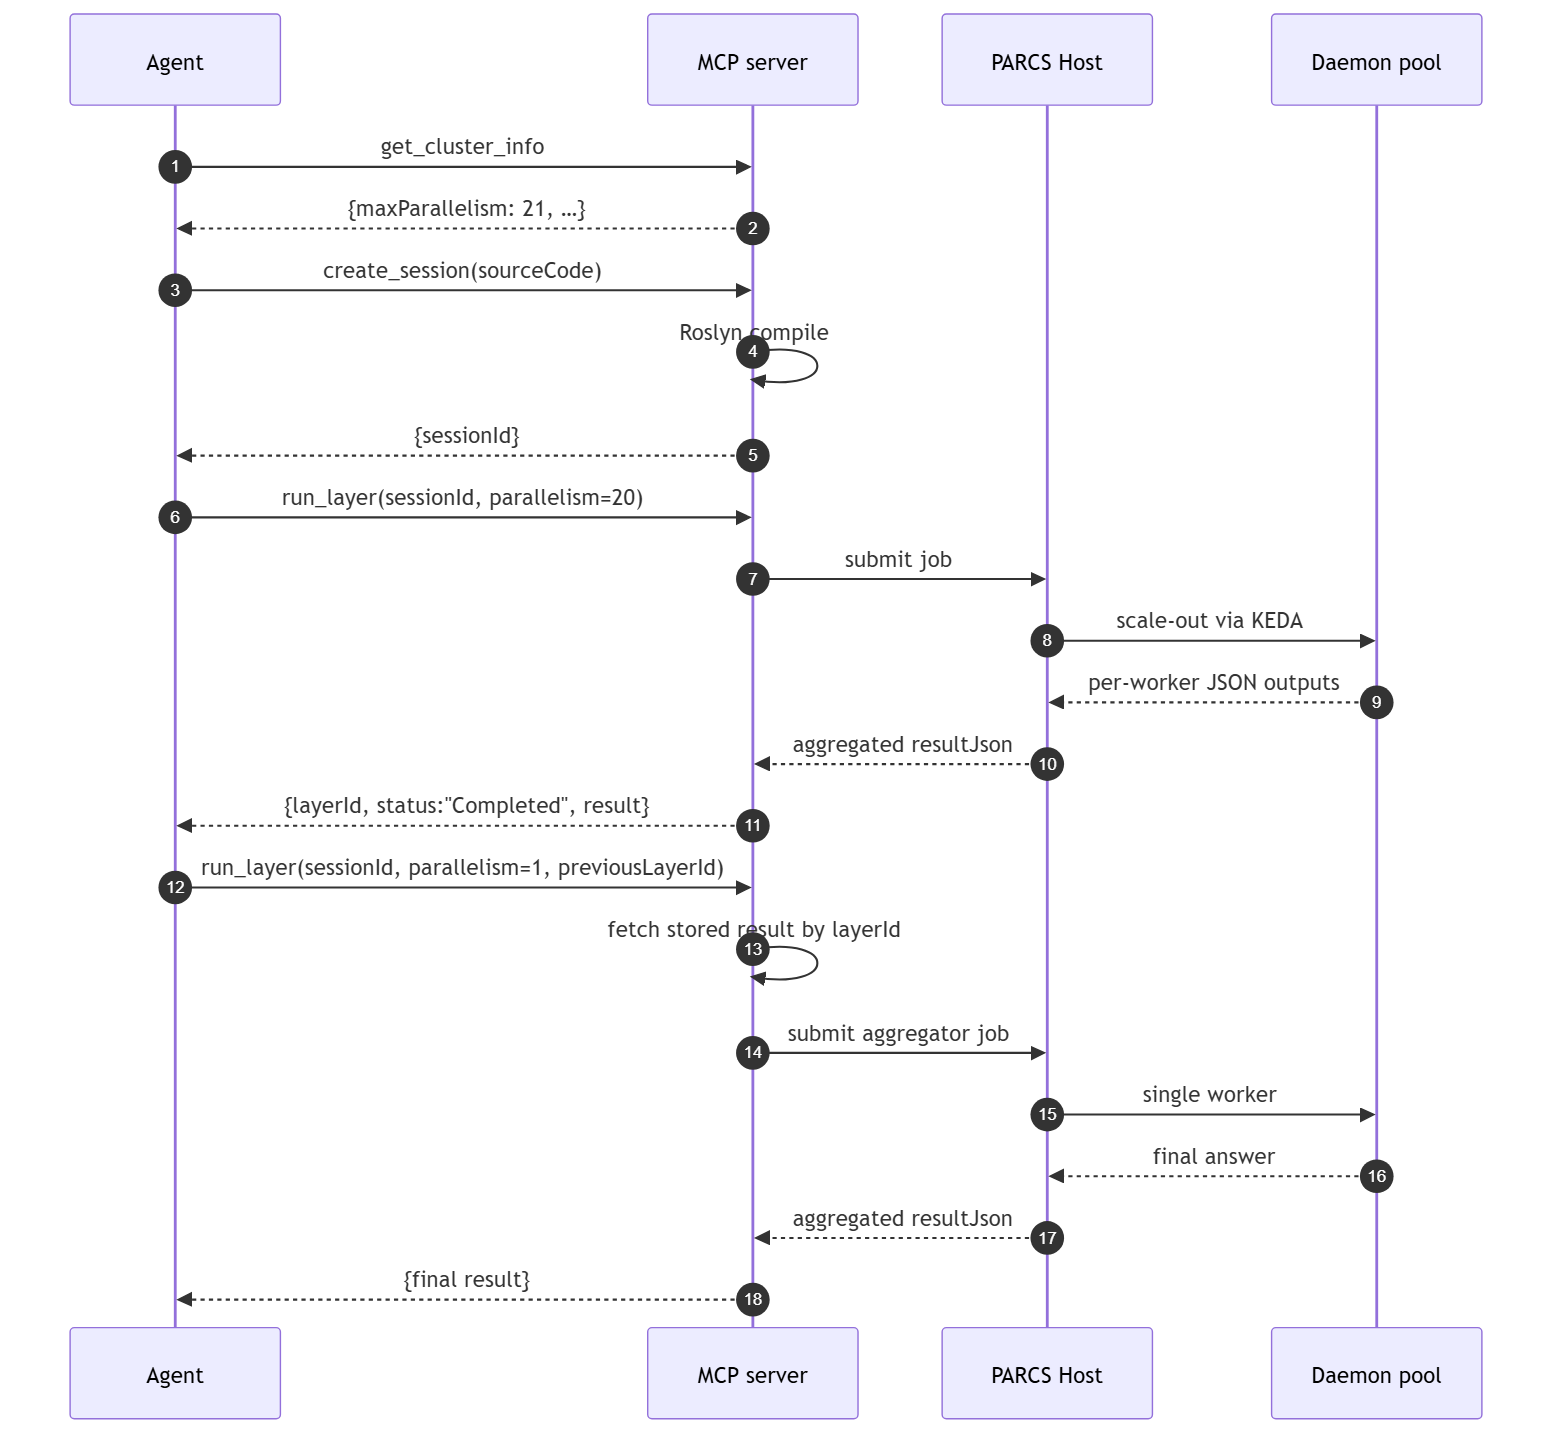
\includegraphics[width=0.85\linewidth]{figures/fig2-sequence}%
}{%
    \fbox{\parbox[c][6em][c]{0.85\linewidth}{\centering\footnotesize\itshape
        [Fig.~2 placeholder --- render \texttt{figures/fig2-sequence.mmd}
        to PNG/PDF and place at \texttt{figures/fig2-sequence.png}]}}%
}
\end{center}
\citfigcaption{2}{%
    \foreignlanguage{ukrainian}{Послідовність двошарового агентного обчислення: виявлення можливостей виконується одноразово; \texttt{create\_session} компілює код агента; \texttt{run\_layer} викликається один раз на шар.}%
}{%
    Sequence of a representative two-layer agent computation. Capability discovery is performed once; \texttt{create\_session} compiles the agent's code; \texttt{run\_layer} is invoked once per layer, with the prior layer's output threaded forward by reference.%
}

\textit{Dataset distribution.}\quad Many agent workloads consume a large shared input such as a covariance matrix, a feature table, or a corpus file. Marshalling such inputs through the protocol replicates the data across workers and burdens the MCP transport. To address this, \texttt{run\_layer} accepts an optional \texttt{datasetUrl} argument. The MCP server downloads the referenced resource once into a content-addressed directory on a shared NFS volume mounted by all daemons at the same path, and exposes that path to each worker via \texttt{input.DatasetPath}. Subsequent layers referencing the identical URL retrieve the file from the local cache without further transfer. The mechanism is transport-agnostic and supports any HTTP-reachable source, including HuggingFace, Google Cloud Storage, Azure Blob Storage, and private object stores.

\textit{Choice of execution language.}\quad PARCS is implemented in .NET, existing modules are distributed as .NET assemblies, and Roslyn provides a JIT-quality compiler accessible from the same process as the MCP server. Using C\# preserves a single compilation and execution stack from agent input to worker output. The choice carries a trade-off: the agent must produce C\# rather than Python, the language more frequently encountered in LLM pre-training data. In practice, frontier models handle the language without measurable quality degradation, in part because the generated code consists of straight-line procedural logic and contains no platform-specific parallel constructs.

\medskip\noindent\textbf{Case study: Monte Carlo Value-at-Risk}\par\nopagebreak
The case considered in this subsection is drawn from a benchmark harness developed alongside the system but reserved for a future evaluation publication. The task is canonical in quantitative finance: estimation of the 1-day 99\,\% Value-at-Risk (VaR) and Conditional Value-at-Risk (CVaR) of a portfolio of 50 equally weighted assets whose return covariance matrix $\Sigma$ is generated from a fixed random seed. The reference protocol specifies $200\,000$ Monte Carlo scenarios distributed across 20 workers at $10\,000$ scenarios each --- a sample count for which a single-threaded sandbox is poorly suited and which is naturally addressed by fan-out across the cluster's worker pool.

The decomposition produced by the agent, following the system-prompt scaffold provided to it, comprises two layers preceded by a capability-discovery call:

\begin{enumerate}[leftmargin=1.5cm,topsep=2pt,itemsep=2pt]
  \item \textbf{Capability discovery.} A single invocation of \texttt{get\_cluster\_info} returns \texttt{maxParallelism}, the upper bound used to size subsequent layers.
  \item \textbf{Layer 1 --- parallel sampling (\texttt{parallelism = 20}).} Each worker draws $10\,000$ Gaussian scenarios using \texttt{new Random(WorkerIndex * 1000 + 42)} together with the shared Cholesky factor of $\Sigma$, computes the per-scenario portfolio loss, and returns its loss vector serialised as JSON.
  \item \textbf{Layer 2 --- aggregation (\texttt{parallelism = 1}).} A second invocation of \texttt{run\_layer} is issued with \texttt{previousLayerId} set to the identifier of layer~1; the server retrieves the stored result, and the single worker reads it from \texttt{input.PreviousLayerResultJson}. The worker concatenates the loss vectors into the full sample of $200\,000$ losses, computes the empirical 99th percentile (the VaR estimate) and the conditional mean above it (the CVaR estimate), and returns \texttt{\{var\_99, cvar\_99\}}.
\end{enumerate}

A representative excerpt of the worker layer is shown below:

\begin{center}
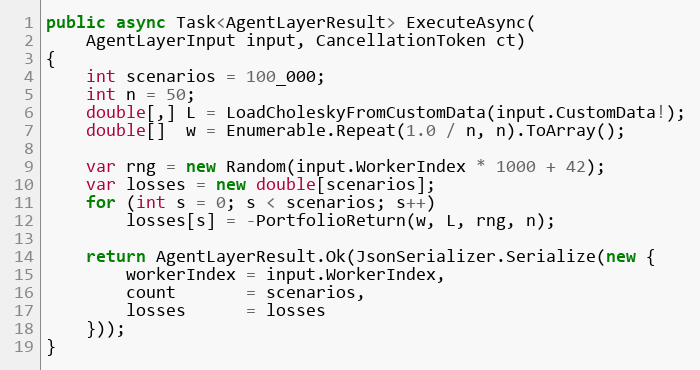
\includegraphics[width=0.85\linewidth]{sources/source1.cs.png}
\end{center}

The implementation contains no synchronisation primitives, no channel construction, and no thread-pool configuration. The worker is functionally equivalent to a single-threaded estimator parameterised by a different random seed. Deterministic per-worker seeding from \texttt{WorkerIndex} ensures disjoint random streams. The output is plain JSON because \texttt{outputData} is a string-typed field at the platform interface.

The case study illustrates four architectural properties of the system.

\begin{enumerate}[leftmargin=1.5cm,topsep=2pt,itemsep=2pt]
  \item \textit{The agent provides only per-worker logic.} Fan-out across 20 workers, the barrier between layers, and the propagation of layer~1's output to layer~2 via \texttt{previousLayerId} are all platform concerns invisible to the agent.
  \item \textit{Aggregation reuses the parallel primitive.} The reducer in layer~2 is a \texttt{run\_layer} invocation with \texttt{parallelism = 1}. The protocol does not distinguish a ``map'' phase from a ``reduce'' phase; \texttt{parallelism} is a numeric parameter rather than a semantic mode.
  \item \textit{Recoverable failure preserves session state.} If the first compilation attempt is rejected --- a realistic occurrence given the difficulty LLMs encounter with C\# numeric generics --- the agent invokes \texttt{create\_session} again with corrected source. The artefacts of the failed compilation are discarded; layer~1 has not yet been executed and no prior work is lost. Should the failure occur during layer~2 instead, the agent retries \texttt{run\_layer} with the same \texttt{previousLayerId}, referencing the still-stored layer~1 result and avoiding re-execution of the sampling step.
  \item \textit{Dataset distribution decouples from worker count.} In an extension where $\Sigma$ is loaded from a multi-megabyte file rather than transmitted as \texttt{customData}, the agent provides a \texttt{datasetUrl} argument on the first \texttt{run\_layer} call. Subsequent layers referencing the same URL incur no additional transport cost regardless of the number of workers.
\end{enumerate}

The case study is not a benchmark and asserts no claim about wall-clock duration or solution quality. Its purpose is to ground the architectural description in concrete agent behaviour and to demonstrate that the synchronous coding paradigm is preserved end-to-end while parallel execution is delivered transparently beneath it.
